\chapter{Resultados}
\label{chap:resultados}

\drop{E}{n} este capítulo se presentan los resultados obtenidos tras llevar a
cabo el plan de trabajo presentado en el capítulo anterior. El proceso ha
desembocado en la obtención de varios artefactos, principalmente SparkDQ y su
prueba de concepto, tal y como se pretendía desarrollar.

\section{Fase de Inicio}

Durante la fase inicial, se destina una iteración a planificar el desarrollo del
\acs{TFM}, establecer requisitos y en función de éstos extraer una serie de
casos de uso.

Las tablas expuestas en el capítulo anterior se van a exponer de nuevo con el
fin de facilitar la lectura.

\subsection{Iteración 1: Planificación, casos de uso y requisitos}

La primera iteración tiene como objetivo establecer una planficación, detallar
requisitos y establecer una serie de casos de uso.

Se han obtenido como resultados los siguientes artefactos:

\begin{itemize}
\item Una revisión del estado del arte que puede consultarse en el Capítulo
  \ref{chap:estadoarte}, reflejando la situación actual en los principales
  campos relacionados con el \acs{TFM}
  \begin{itemize}
  \item Web Semántica
  \item Procesamiento en distribuido
  \item Calidad de Datos
  \item Calidad de Linked Data
  \end{itemize}

\item Una especificación de requisitos, funcionales y no funcionales, tanto para
  SparkDQ como para la prueba de concepto a realizar a partir de ésta.
\item Modelo general de Casos de Uso de SparkDQ y \acs{PoC}
\item Planificación detallada dividida en fases e iteraciones del \acs{PUD}
\end{itemize}

% Iteración 1
\vspace{1cm}
\begin{tabular}{|p{.4\textwidth}|p{.4\textwidth}|}

\hline

\cellcolor[gray]{0.7}Fase del \acs{PUD} & Inicio 
 \\
\hline

\cellcolor[gray]{0.7}Flujo de trabajo del \acs{PUD} & Análisis y Diseño
 \\
\hline

\cellcolor[gray]{0.7}Objetivos  &
\cellcolor[gray]{0.7}Artefactos de Salida \\
\hline

\begin{itemize}
\item Contextualizar trabajo \acs{PFC}
\item \acs{CdU} iniciales y requisitos
\item Arquitectura preliminar
\end{itemize}

&

\begin{itemize}
\item Plan de actualización artefactos \acs{PFC}
\item Diagrama \acs{CdU} y \acf{RF}
\item Arquitectura preliminar
\end{itemize} \\
\hline
\end{tabular}
\captionof{table}{Iteración 1: Fase de Inicio}


% Local variables:
%   coding: utf-8
%   ispell-local-dictionary: "castellano8"
%   TeX-master: "main.tex"
% End:


\subsubsection{Requisitos}

Los requisitos funcionales de cualquier sistema software son aquellos que definen el comportamiento del
sistema y establecen un punto de partida para elaborar un modelo de casos de
uso (ver figura \ref{fig:cdu-general}), mientras que los no funcionales son aquellos orientados a aspectos del
sistema que notienen relación con el comportamiento, por ejemplo, el diseño, la
implementación on la usabilidad. 

Seguidamente se exponen los requisitos funcionales que se han identificado en la
primera fase del \acs{PUD}. Estos requisitos corresponden al desarrollo del
stack \textbf{SparkDQ}.

\begin{enumerate}
\item \textbf{RF 1. SparkDQ debe permitir la carga de triplas semánticas en un entorno
  distribuido} \\La premisa inicial es que el volumen de datos es
  suficientemente grande como para que se requiera un almacenamiento y
  procesamiento en distribuido de los mismos. Por lo tanto, SparkDQ debe ser
  capaz de leer las triplas almacenadas en entornos distribuidos y cargarlas en
  un modelo igualmente distribuido para su posterior procesamiento.
  
\item \textbf{RF 2. SparkDQ debe permitir al usuario modelar la evaluación de
  calidad}\\Se entiende como evaluación de calidad el cálculo de unas métricas y
  su posterior interpretación, así pues SparkDQ debe exponer mecanismos de
  evaluación de calidad de datos para ser llevados a cabo sobre un juego de
  datos distribuido. 
\item \textbf{RF 3. SparkDQ debe permitir llevar a cabo evaluaciones de calidad de
  datos enlazados para la métrica \textit{SchemaCompleteness}}\\Se evaluará esta
  métrica considerando un esquema deseable para los datos obteniendo como
  resultado un grado de alineamiento de los datos con dicho esquema. 

\item \textbf{RF 4. SparkDQ debe permitir llevar a cabo evaluaciones de calidad de
  datos enlazados para la métrica \textit{InterlinkingCompleteness}}\\Se
  evaluará esta métrica considerando un nivel de profundidad, siendo esto una
  agregación del nivel de interconectividad estratificado. 
\end{enumerate}

Una vez definidos los funcionales, se indican los no funcionales para SparkDQ.

\begin{itemize}
\item \textbf{RNF 1. Utilización de un framework para desarrollo de tecnologías
  semánticas: Apache Jena}\\Se retomará el uso de Apache Jena como framework de
  desarrollo de tecnologías semánticas para utilizar en el contexto del \acs{TFM}
\item \textbf{RNF 2. Utilización de un framework de procesamiento en
  distribuido: Apache Spark}\\Para el procesamiento distribuido se utilizará
  Apache Spark, que queda explicado en la sección \ref{sec:eco-hadoop}
\item \textbf{RNF 3. Generación de la documentación de la \acs{API}}\\Finalmente
  se generará la documentación de la API que permita a los desarrolladores
  extender y utilizar el módulo creado. 
\end{itemize}

Finalmente se exponen los requisitos funcionales y no funcionales identificados para la
aplicación de Prueba de Concepto.

\begin{enumerate}
\item \textbf{\acs{PoC} debe permitir la adquisición de datos semánticos}\\Como parte
  del \textit{end to end} el primer paso de la prueba de concepto será
  seleccionar una fuente de datos y llevar a cabo un proceso de ingesta dentro
  de la arquitectura propuesta. 
  
\item \textbf{\acs{PoC} debe permitir el almacenamiento de datos semánticos en un
  entorno distribuido}\\Los datos deben ingestarse en un entorno distribuido
  para su posterior consumo, considerando que su volumen y variedad pueden
  cambiar a lo largo del tiempo. 
\item \textbf{\acs{PoC} debe permitir cargar datos semánticos desde un entorno
  distribuido y procesarlos}\\Los datos almacenados deben ser fácilmente
  accesibles y consumidos, entendiendo el consumo de estos datos como la
  adquisición, procesamiento y obtención de resultados en base a éstos. 
\item \textbf{\acs{PoC} debe mantener unos niveles de seguridad adecuados}\\Los datos
  ingestados y almacenados deben estar protegidos de accesos no deseados. 
\item \textbf{\acs{PoC} debe poder almacenar el resultado de las evaluaciones de
  calidad de datos en un entorno distribuido}\\Los resultados de las
  evaluaciones deben ser convenientemente almacenados bajo las mismas
  directrices de disponibilidad y seguridad que los datos inicialmente ingestados.
\item \textbf{\acs{PoC} debe permitir el consumo de los resultados de las evaluaciones
  llevadas a cabo}\\Los resultados de las evaluaciones deben ser accesibles y
  fácilmente consumibles por parte de los usuarios. 
\end{enumerate}

Siendo los requisitos no funcionales los siguientes:

\begin{itemize}
\item \textbf{RNF 1. Arquitectura en Cloud}\\Se debe realizar una prueba de
  concepto utilizando tecnologías Cloud recientes y de uso extendido. 

\item \textbf{RNF 2. Utilización de parte del ecosistema Apache}\\Siendo SparkDQ
  un incremento sobre un framework del ecosistema Hadoop, se buscará integrarse
  también con otras tecnologías del mismo ecosistema. 
\end{itemize}


\subsubsection{Modelo general de Casos de Uso}

Uno de los primeros pasos consiste en la elaboración del modelo de Casos de Uso
para el proyecto. 

Se han identificado dos sistemas, SparkRDF y SparkDQ, con dependencia de éste
último sobre el primero, conteniendo ambos los casos que se ilustran y se
detallarán en las iteraciones pertinentes (secciones \ref{iteracion4} y \ref{iteracion5}). 

El modelo general se puede consultar en la figura \ref{fig:cdu-general}.

\begin{figure}[!h]
  \begin{center}
    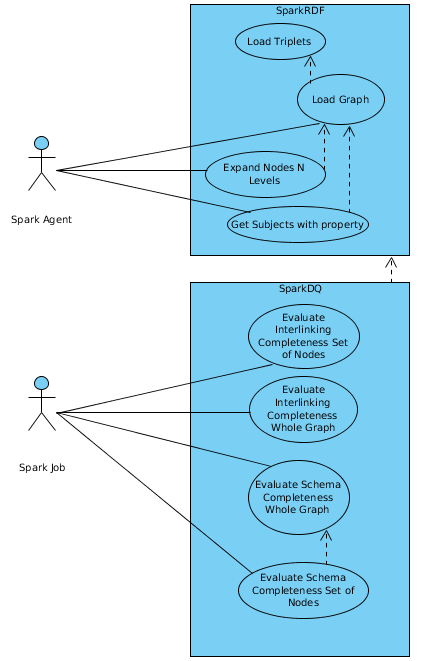
\includegraphics[width=0.6\textwidth]{cdu-general.png} 
    \caption{Diagrama general de Casos de Uso}
    \label{fig:cdu-general}
  \end{center}
\end{figure}



\section{Fase de Elaboración}

En la fase de Elaboración, se han sentado las bases para el desarrollo
propiamente dicho de los artefactos software que se han indicado en la fase
inicial. Concretamente se ha trabajado en dos vertientes:

\begin{itemize}
\item Actualización de JenaDQ como artefacto software
\item Diseño del stack SparkDQ
\end{itemize}

\subsection{Iteración 2: Actualización de JenaDQ}

% Iteración 2
\vspace{1cm}
\begin{tabular}{|p{.4\textwidth}|p{.4\textwidth}|}

\hline

\cellcolor[gray]{0.7}Fase del \acs{PUD} & Elaboración
 \\
\hline

\cellcolor[gray]{0.7}Flujo de trabajo del \acs{PUD} & Análisis, Diseño, Implementación y Pruebas
 \\
\hline



\cellcolor[gray]{0.7}Objetivos  &
\cellcolor[gray]{0.7}Artefactos de Salida \\
\hline

\begin{itemize}
\item Actualización JenaDQ
\end{itemize}

&

\begin{itemize}
\item JenaDQ actualizado
\end{itemize}
 \\
\hline
\end{tabular}
\captionof{table}{Iteración 2: Actualización de JenaDQ}


% Local variables:
%   coding: utf-8
%   ispell-local-dictionary: "castellano8"
%   TeX-master: "main.tex"
% End:


En esta iteración el objetivo principal es actualizar JenaDQ y alinearlo con las
tecnologías que van a ser usadas en este proyecto.

Concretamente, se ha generado
un proyecto Maven (véase Sección\ref{maven}) con el que gestionar más fácilmente
las dependencias y el ciclo de vida de las aplicación.

Posteriormente se ha hecho una revisión del código y se han actualizado aquellos
puntos de JenaDQ que se han creído oportunos:

\begin{enumerate}
\item Se han añadido más pruebas unitarias.
\item Refactorizado de código.
\item Test de integración.
\end{enumerate}

Como resultado se ha obtenido una nueva versión de JenaDQ, que ha mantenido las
métricas pero cuyo nivel de calidad como artefacto software y mantenibilidad se
ha visto incrementado.

\subsection{Iteración 3: Diseño de la arquitectura de SparkDQ}
\label{iteracion3}
% Iteración 3
\vspace{1cm}
\begin{tabular}{|p{.4\textwidth}|p{.4\textwidth}|}

\hline

\cellcolor[gray]{0.7}Fase del \acs{PUD} & Elaboración
 \\
\hline

\cellcolor[gray]{0.7}Flujo de trabajo del \acs{PUD} & Análisis y Diseño

 \\
\hline


\cellcolor[gray]{0.7}Objetivos  &
\cellcolor[gray]{0.7}Artefactos de Salida \\
\hline

\begin{itemize}
\item Diseñar nueva arquitectura de framework
\item Diserñar arquitectura PoC
\end{itemize}

&

\begin{itemize}
\item Diseño de SparkRDF y SparkDQ
\item Diseño de \acs{PoC} preliminar
\end{itemize}

 \\
\hline
\end{tabular}
\captionof{table}{Iteración 3: Diseño de soluciones }


% Local variables:
%   coding: utf-8
%   ispell-local-dictionary: "castellano8"
%   TeX-master: "main.tex"
% End:


La iteración ha tenido como objetivo:

\begin{itemize}
\item Establecer un diseño de la arquitectura de SparkDQ
\item Establecer un diseño de la arquitectura de la prueba de concepto
\end{itemize}

En primer lugar se ha concluido que SparkDQ contará con dos elementos:
\begin{itemize}
\item \textbf{SparkRDF}: un artefacto encargado únicamente de la captura de datos
  semánticos y su transformación a una estructura de datos distribuida. En este
  caso, dicha estructura será la de un grafo dirigido. Este grafo se construirá
  sobre la librería Spark GraphX, orientada específicamente a trabajar con este
  tipo de estructuras.
  \item \textbf{SparkDQ}: artefacto encargado de llevar a cabo evaluaciones de
    calidad de datos sobre datos semánticos. Tendrá una dependencia con
    SparkRDF, delegando en éste la adquisición de datos y tomando en sus
    funciones como puntos de entrada los datos extraídos por SparkRDF. Se
    plantean a su vez dos métricas para evaluar: \textit{Interlinking} y
    \textit{SchemaCompleteness}, descritas en la sección \ref{schemacompleteness}. 
\end{itemize}

Para la prueba de concepto, se ha establecido:

\begin{enumerate}
\item Generación de un artefacto que lleve a cabo cálculos de calidad de datos
  semánticos sobre un conjunto suficientemente grande. Dicho artefacto se
  llamará spark-sem-dq-assessment y tendrá una dependencia de SparkDQ. Podrá
  configurarse para llevar a cabo una evaluación de la calidad de los datos
  sobre cualquiera de las métricas que ofrezca SparkDQ.
\item Elaboración de un diseño de arquitectura en cloud: involucrará los
  siguientes elementos:
  \begin{enumerate}
  \item Arquitectura de microservicios: para llevar a cabo la captura y
    procesamiento de datos. 
  \item Almacenamiento en cloud - Amazon S3: como repositorio de datos iniciales
    y directorio final de resultados de cálculos.
  \item Visualización - Amazon ElasticSearc and Kibana stack: para la
    visualización de los resultados de las evaluaciones.  
  \end{enumerate}
\end{enumerate}

Se ha obtenido como resultado el diagrama de clases de SparkRDF, diagrama de clases
de SparkDQ (figura \ref{fig:classes}) y diagrama de componentes de la prueba de
concepto (figura \ref{fig:sequence-aws}).

\begin{figure}[!h]
  \begin{center}
    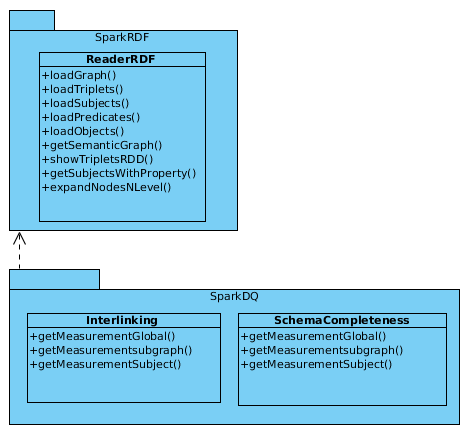
\includegraphics[width=0.8\textwidth]{classes.png} 
    \caption{Diagrama de clases SparkDQ}
    \label{fig:classes}
  \end{center}
\end{figure}

\begin{figure}[!h]
  \begin{center}
    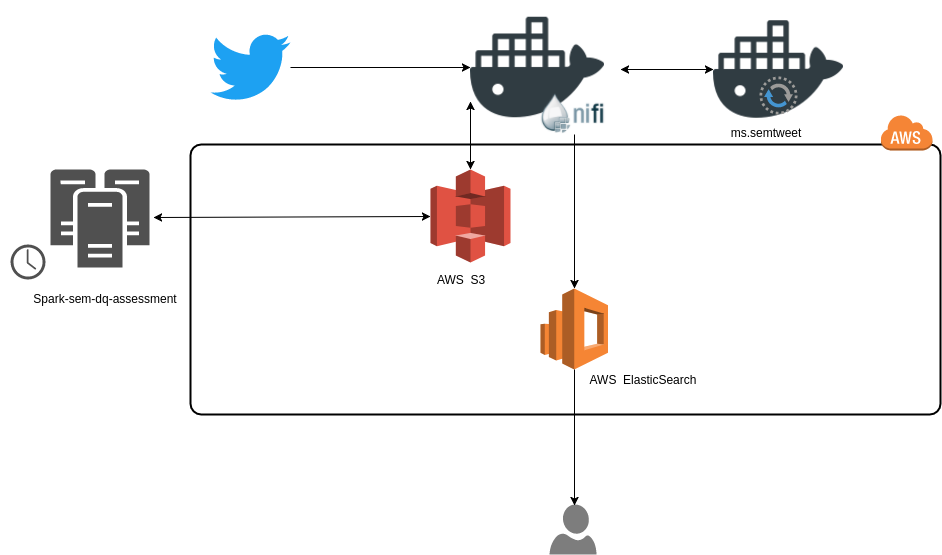
\includegraphics[width=1.0\textwidth]{PoC.png} 
    \caption{Diagrama de componentes para la \acs{PoC}}
    \label{fig:sequence-aws}
  \end{center}
\end{figure}


\section{Fase de Construcción}

Una vez asentados los diseños de los artefactos a desarrollar, en la fase de
construcción tendrá lugar el desarrollo del núcleo de la aplicación, esto es,
los artefactos clave de desarrollo: SparkRDF y SparkDQ, en las iteraciones 4 y 5
respectivamente. Se considera el ciclo completo de desarrollo en estos puntos:
Análisis, Diseño, Implementación y Pruebas. Dichas pruebas tendrán lugar en la
fase final como parte de un paso de \acf{QA}, y serán indicativas sobre la
repetición del ciclo en caso de que los resultados no sean los esperados. 

\subsection{Iteración 4: Desarrollo de SparkRDF}
\label{iteracion4}
% Iteración 4
\vspace{1cm}
\begin{tabular}{|p{.4\textwidth}|p{.4\textwidth}|}

\hline

\cellcolor[gray]{0.7}Fase del \acs{PUD} & Elaboración
 \\
\hline

\cellcolor[gray]{0.7}Flujo de trabajo del \acs{PUD} & Análisis, Diseño,
Implementación y Pruebas
 \\
\hline


\cellcolor[gray]{0.7}Objetivos  &
\cellcolor[gray]{0.7}Artefactos de Salida \\
\hline

\begin{itemize}
\item Desarrollo de SparkRDF
\item Primitivas de lectura de triplas y exportar a modelo distribuido
\item \acs{QA}
\item Documentación SparkRDF
\end{itemize}

&

\begin{itemize}
\item Artefacto SparkRDF
\item Documentación SparkRDF
\end{itemize}
\\
\hline
\end{tabular}
\captionof{table}{Iteración 4: Desarrollo de SparkRDF}


% Local variables:
%   coding: utf-8
%   ispell-local-dictionary: "castellano8"
%   TeX-master: "main.tex"
% End:


SparkRDF utiliza un sub-módulo de Apache Jena (riot) para la lectura de
documentos en formato \texttt{TTL} o \texttt{NT}, es decir, en forma de triplas, en las que cada línea
del fichero tiene tres campos separados por espacio, siendo dichos campos sujeto,
predicado y objeto, respectivamente. El listado \ref{rdflector} muestra un
fragmento de código encargado de la lectura de triplas y almacenamiento en un
RDD. 

\lstset{escapechar=@,language=scala}
\begin{lstlisting}[caption={Fragmento del lector de triplas},captionpos=b, label=rdflector]
def loadTriplets(sparkSession: SparkSession, path: String): RDD[Triple] = {
  val tripletsRDD = sparkSession.sparkContext.textFile(path)
  .filter(line => !line.trim().isEmpty & !line.startsWith(``#''))
  .map(line =>
          RDFDataMgr.createIteratorTriples(new
          ByteArrayInputStream(line.getBytes), Lang.NTRIPLES, null).next())
          tripletsRDD
}  
\end{lstlisting}

Una vez cargadas las triplas y puesto que la información semántica es
inherentemente un grafo, se utiliza la extensión GraphX de Spark para generar un
grafo dirigido de triplas semánticas, en el que los nodos son sujetos y objetos y los
arcos son las relaciones entre los nodos. El listado \ref{graphcomposer} ilustra
esta funcionalidad. 

\lstset{escapechar=@,language=scala}
\begin{lstlisting}[caption={Conversión de RDD de Triplas a Grafo de nodos},captionpos=b, label=graphcomposer]
private def getSemanticGraph(tripleRDD: RDD[Triple]): org.apache.spark.graphx.Graph[Node, Node] = {
//Generate hashCodes for graphx representation
    val extTripleRDD = tripleRDD.map(triple => (triple,
        triple.getSubject().hashCode().toLong,
        triple.getObject().hashCode().toLong))
    val subjects: RDD[(VertexId, Node)] = tripleRDD.map(triple =>
        (triple.getSubject().hashCode().toLong, triple.getSubject()))
    val predicates: RDD[Edge[Node]] = extTripleRDD.map(line =>
        Edge(line._2, line._3, line._1.getPredicate()))
    val objects: RDD[(VertexId, Node)] = tripleRDD.map(triple =>
        (triple.getObject().hashCode().toLong, triple.getObject()))
    val graph = org.apache.spark.graphx.Graph(subjects.union(objects).distinct(),
         predicates.distinct())
    graph
}
\end{lstlisting}

El tratamiento de los datos RDF y por ende las responsabilidades de este
artefacto no terminan solamente con la lectura y transformación a una estructura
de grafo distribuida, sino que cualquier operación de tratamiento y consulta de
estos datos debe delegar en esta capa de abstracción. Así pues, además de las
nombradas, existe una serie de funciones dedicadas a llevar a cabo operaciones
auxiliares sobre un conjunto de triplas, tales como listar sujetos, predicados,
objetos o funciones de consulta como las de buscar nodos que cumplan cierta
propiedad. 

Como se verá en la siguiente sección, existe una función clave para el
desarrollo de este proyecto y el cálculo de las métricas, que queda delegada a
SparkRDF:

\lstset{escapechar=@,language=scala}
\begin{lstlisting}[caption={Conversión de RDD de Triplas a Grafo de
      nodos},captionpos=b, label=headerexpand]

def expandNodesNLevel(nodes: VertexRDD[Node],
                        graph: org.apache.spark.graphx.Graph[Node, Node],
                        levels: Int = 1): Dataset[Row]   
\end{lstlisting}

Su funcionalidad es la de, dada una colección de nodos, expandir en N capas esos
nodos. En la siguiente sección se explicará en detalle la necesidad de esta
funcionalidad. 

\subsection{Iteración 5: Desarrollo de SparkDQ para la métrica \textit{Interlinking}}
\label{iteracion5}
% Iteración 5

\begin{tabular}{|p{.4\textwidth}|p{.4\textwidth}|}

\hline

\cellcolor[gray]{0.7}Fase del \acs{PUD} & Elaboración
 \\
\hline

\cellcolor[gray]{0.7}Flujo de trabajo del \acs{PUD} & Análisis, Diseño,
Implementación y Pruebas
 \\
\hline

\cellcolor[gray]{0.7}Fechas Inicio - Fin  &
 \\
\hline

\cellcolor[gray]{0.7}Objetivos  &
\cellcolor[gray]{0.7}Artefactos de Salida \\
\hline

\begin{itemize}
\item Desarrollo de SparkDQ
\item Métrica Interlinking
\item QA
\end{itemize}

&

\begin{itemize}
\item Artefacto SparkDQ preliminar con primera métrica
\end{itemize}
\\
\hline
\end{tabular}
\captionof{table}{Iteración 5}


% Local variables:
%   coding: utf-8
%   ispell-local-dictionary: "castellano8"
%   TeX-master: "main.tex"
% End:


Se define la métrica \textit{Interlinking} como el índice en el que las
instancias en el conjunto de datos están interconectadas, entendiendo
interconexión como el \textit{grado} para un determinado nodo del grafo. No
obstante, se particulariza en el ámbito de los datos enlazados, como el índice de
conexiones que tiene dicho nodo hacia nodos que no sean hoja, es decir, sigan
siendo nodos desreferenciables y así tengan un grado mayor a cero. Así,
para un nodo, se pueden establecer métricas de
interconexión por niveles:

\begin{itemize}
\item Nivel 0: los vecinos directos del nodo: V1 
\item Nivel 1: Para cada nodo perteneciente a V1, el conjunto unión de todos sus
  vecinos: V2
\item etc. 
\end{itemize}

De esta manera se obtiene una métrica estratificada por niveles. Así, para cada nivel, se
tendría el número de nodos que son URIs respecto del total de vecinos directos. 

Para abordar esta métrica se distinguen dos fases: 

\begin{enumerate}
\item Para todos los nodos, es decir, sujetos semánticos candidatos a calcular
  la métrica, expandir por niveles para conocer los nodos con los que está
  relacionado tal y como se ha explicado en el punto anterior. Se ilustra el
  algoritmo en el listado \ref{graphexpandN}. 

\item Formar una tabla con las siguientes entradas: 
  \begin{itemize}
  \item Id del nodo sujeto (\texttt{Nodo})
  \item Profundidad N (\texttt{Int})
  \item Nodo vecino en profundidad N (\texttt{Nodo})
  \item Nodo vecino en profundidad N es URI (\texttt{Boolean})
  \end{itemize}
\item Sobre esta estructura, agrupar por Id del nodo/profundidad contando el
  número de nodos que son URI y dividiendo entre el total por el nivel. De esta
  manera se obtiene un número entre 0 y 1 correspondiente a la métrica para ese
  sujeto. Véase listado \ref{graphmetric}.
\end{enumerate}

\lstset{escapechar=@,language=scala}
\begin{lstlisting}[caption={Expansión de nodos en N niveles para un conjunto de
      sujetos},captionpos=b, label=graphexpandN]

  def expandNodesNLevel(nodes: VertexRDD[Node],
                        graph: org.apache.spark.graphx.Graph[Node, Node],
                        levels: Int = 1): Dataset[Row] = {
    import processSparkSession.implicits._

    val edges = graph.edges.map(l => (l.srcId, l.dstId)).toDF(Seq(``srcId'',
    ``dstId''): _*).cache()
    var edgesR = graph.edges.map(l => (l.srcId, l.dstId,
    0)).toDF(Seq(``source'', ``level'', ``depth''): _*).cache()
    val nodesR = nodes.map(l => l._1).toDF(Seq(``nodeId''): _*)

    var results = edgesR.distinct()

    for (level <- 1 until levels) {
      val res = edges.join(edgesR.drop(``depth''), $''dstId'' === $''source'',
      ``leftouter'').orderBy($''srcId'')
      edgesR = res.select($''srcId'' as ``source'', $''level'' as
      ``level'').withColumn(``depth'', lit(level))
      results = results.union(edgesR.distinct())
    }
    results = results.join(nodesR, $''source'' ===
    $''nodeId'').drop($''nodeId'').na.drop().distinct().orderBy($''depth'',
    $''source'')
    results
  }
}

\end{lstlisting}

\lstset{escapechar=@,language=scala}
\begin{lstlisting}[caption={Cálculo de la métrica en colección expandida de nodos},captionpos=b, label=graphmetric]
  def getMeasurementSubgraph(subjects: VertexRDD[Node], graph: Graph[Node,
    Node], depth: Int ): Dataset[Row] = {
    val expanded = expandNodesNLevel(subjects, graph, depth)
    import processSparkSession.implicits._
    val subs = subjects
      .filter(ll => ll._2.isURI())
      .map(l => (l._1, l._2.getURI())).toDF(Seq(``vertexId'', ``vertexURI''):
    _*)
    val filteredNodes = graph.vertices.map(l => (l._1,
    l._2.isURI())).toDF(Seq(``nodeId'', ``isURI''): _*)
    val nodesTF = expanded.join(filteredNodes, $''level'' ===
    $''nodeId'').drop($''nodeId'').drop($''level'').orderBy($''source'',
    $''depth'')
    val partResultTrue = nodesTF.groupBy($''source'',
    $''depth'').agg(count(when($''isURI'' === true, true)) as
    ``countT'').orderBy($''source'', $''depth'')
    val partResultFalse = nodesTF.groupBy($''source'',
    $''depth'').agg(count(when($''isURI'' === false, true)) as
    ``countF'').orderBy($''source'', $''depth'')
      .toDF(Seq(``sourceF'', ``depthF'', ``countF''): _*)
    val result = partResultTrue.join(partResultFalse, $''source'' ===
    $''sourceF'' and $''depth'' ===
    $''depthF'').drop($''sourceF'').drop($''depthF'').orderBy($''source'',
    $''depth'')
      .withColumn(``measurement'', getRatio($''countT'',
    $''countF'')).join(subs, $''source'' === $''vertexId'').drop($''vertexId'')
    result
  }
\end{lstlisting}

Finalmente se acaba la iteración con las pruebas correspondientes a la
funcionalidad desarrollada. 


\subsubsection{Ejemplo}

El siguiente ejemplo ilustra el cálculo de la métrica Interlinking para el
grafo que se muestra a continuación. Los datos con los que se ha tomado este
ejemplo pueden consultarse en el apéndice \ref{ex:interlinking}.

\begin{listing}[
  language = scala,
  numbers=left,
  numberstyle=\tiny,
  stepnumber=5,
  numbersep=5pt,
  frame=single,
  caption  = {SparkDQ: Interlinking. Ilustración.},
  label    = code:sparkdq.inter.ilus]


//Graph
//    A -> B -> D -> F -> G
//         | \  |
//         v  \,v
//         C -> E
//
// countT: number of URI nodes
// countF: number of literal nodes
//
//      +---------+-----+------+------+-------------------+
//      |   source|depth|countT|countF|        measurement|
//      +---------+-----+------+------+-------------------+
//      |A        |    0|     1|     3|               0.25|
//      |A        |    1|     3|     3|                0.5|
//      |A        |    2|     2|     9|0.18181818181818182|
//      |A        |    3|     1|     6|0.14285714285714285|
//      |B        |    0|     3|     3|                0.5|
//      |B        |    1|     2|     9|0.18181818181818182|
//      |B        |    2|     1|     6|0.14285714285714285|
//      |B        |    3|     0|     3|                0.0|
//      |C        |    0|     1|     3|               0.25|
//      |C        |    1|     0|     3|                0.0|
//      |D        |    0|     2|     3|                0.4|
//      |D        |    1|     1|     6|0.14285714285714285|
//      |D        |    2|     0|     3|                0.0|
//      |E        |    0|     0|     3|                0.0|
//      |F        |    0|     1|     3|               0.25|
//      |F        |    1|     0|     3|                0.0|
//      |G        |    0|     0|     3|                0.0|
//      +---------+-----+------+------+-------------------+

\end{listing}
\subsection{Iteración 6: Desarrollo de SparkDQ para la métrica \textit{SchemaCompleteness}}
\label{iteracion6}


% Iteración 6
\vspace{1cm}
\begin{tabular}{|p{.4\textwidth}|p{.4\textwidth}|}

\hline

\cellcolor[gray]{0.7}Fase del \acs{PUD} & Elaboración
 \\
\hline

\cellcolor[gray]{0.7}Flujo de trabajo del \acs{PUD} & Análisis, Diseño,
Implementación y Pruebas
 \\
\hline

\cellcolor[gray]{0.7}Fechas Inicio - Fin  &
 \\
\hline

\cellcolor[gray]{0.7}Objetivos  &
\cellcolor[gray]{0.7}Artefactos de Salida \\
\hline

\begin{itemize}
\item Desarrollo de SparkDQ
\item Métrica SchemaCompleteness
\item \acs{QA}
\end{itemize}

&

\begin{itemize}
\item Artefacto SparkDQ preliminar con segunda métrica
\end{itemize}
\\
\hline
\end{tabular}
\captionof{table}{Iteración 6}


% Local variables:
%   coding: utf-8
%   ispell-local-dictionary: "castellano8"
%   TeX-master: "main.tex"
% End:


Se define la métrica \textit{SchemaCompleteness} como el grado en el que las
clases y propiedades de una ontología están representadas. 

Por lo
tanto, dado un conjunto de propiedades o relaciones entre sujetos y objetos, la
métrica se computa como el ratio de relaciones que un determinado sujeto tiene
con otras entidades. 

En este particular no tiene sentido especificar un grado de esta métrica
estratificado por niveles del grafo puesto que cada nodo vecino del inicial ya
será una entidad en sí mismo, y la métrica aplicada para ese nodo en ese nivel
corresponde únicamente a ese sujeto. Se puede enunciar formalmente así: 

Sea G un grafo formado por un conjunto de nodos N y un conjunto de arcos A. Sea PD un conjunto de propiedades deseables. El valor de la
métrica vendrá dado por el número de propiedades de PD que se
encuentran reflejados en A, dividido entre el número total de propiedades
deseables. 

El cálculo de esta métrica requiere de una serie de pasos que se van a ilustrar
en los siguientes listados. 

\begin{itemize}
\item En primer lugar, se define una función que calcula el valor de la métrica en sí
mismo, esto es, el ratio entre el total de relaciones para un nodo que están
incluídas en la lista de propiedades. Esta función se muestra en el listado
\ref{graphmetricRatio}. Cabe destacar la secuencia de control de la métrica para
valores mayores que 1. Pueden darse en el caso de que un nodo esté conectado con
otros a través de la misma propiedad más de una vez, por ello es importante
considerar que para la métrica tiene efecto la aparición una única vez de la
propiedad. 
\item Seguidamente, se generaliza el cálculo de la métrica para todo el grafo,
ilustrado en el listado \ref{graphmetricSCglobal}. Para
cada propiedad deseable, se obtiene un conjunto de arcos que representan dicha
propiedad. La unión de estos conjuntos es el conjunto de arcos de todo el
grafo, que cumple con todas las propiedades deseables. 
\item El conjunto total de arcos es combinado con el conjunto de arcos que cumplen las
propiedades. Agregando los resultados y contando el total de arcos y de
propiedades. 
\item Aplicando la función inicial para cada nodo del grafo, se obtiene la métrica
global para todos los nodos. 
\item En el paso final, se filtran los nodos del grafo para los nodos candidatos que
quieran evaluarse, como se muestra en el listado \ref{graphmetricSC}.

\end{itemize}

\lstset{escapechar=@,language=scala}
\begin{lstlisting}[caption={Cálculo del ratio},captionpos=b, label=graphmetricRatio]
  def getRatio = udf((totalTrues: Int, total: Int) => {
    var res = totalTrues.toDouble/total.toDouble
    if (res > 1.0)
      res = 1.0
    res
  })
\end{lstlisting}


//TODO IN CODE: filtro en propIdsRDD para hacer distinct de propiedades. 

\lstset{escapechar=@,language=scala}
\begin{lstlisting}[caption={Cálculo de la métrica en el grafo},captionpos=b, label=graphmetricSCglobal]

  def getMeasurementGlobal(graph: Graph[Node, Node], properties: Seq[String]):
  Dataset[Row] = {
    import processSparkSession.implicits._
    val edgeRDD = graph.edges.filter(l => true)

    val propIdsRDD = properties.map(p => edgeRDD.filter(l =>
    l.attr.hasURI(p))).reduce(_ union _)
    //TODO toDF().distinct by srcId, attr.URI(bla)
      .map(l => l.srcId).cache()


    val nonPropsDF = edgeRDD.map(l => l.srcId).toDF(Seq(``source''): _*)
    nonPropsDF.join(propIdsRDD
      .toDF(Seq(``sourceProp''): _*)
      .groupBy($''sourceProp'').agg(count($''sourceProp'') as ``propCount'')
      .withColumn(``totalProperties'', lit(properties.length))
      .withColumn(``meas'', getRatio($''propCount'', $''totalProperties''))
      .drop($''propCount'')
      .drop($''totalProperties'')
      .drop($''srcId''), $''source'' === $''sourceProp'', ``leftouter'')
      .drop($''sourceProp'')
        .withColumn(``measurement'', when(
          col(``meas'').isNull, 0.0
        ).otherwise(col(``meas'')))
      .drop($''meas'')
      .distinct()
  }

\end{lstlisting}
\lstset{escapechar=@,language=scala}
\begin{lstlisting}[caption={Cálculo de la métrica en colección de nodos},captionpos=b, label=graphmetricSC]

  def getMeasurementSubgraph(subjects: VertexRDD[Node], graph: Graph[Node,
    Node], properties: Seq[String]): Dataset[Row] = {
    import processSparkSession.implicits._
    val subjectsDF = subjects
      .filter(ll=> ll._2 != null)
      .filter(l => l._2.isURI())
      .map(l => (l._1, l._2.toString()))
      .toDF(Seq(``srcId'', ``uri''): _*)
    getMeasurementGlobal(graph, properties).join(subjectsDF, $''source'' ===
    $''srcId'')
      .drop($''srcId'')
  }

\end{lstlisting}

Finalmente se acaba la iteración con las pruebas correspondientes a la
funcionalidad desarrollada. 

\subsubsection{Ejemplo}

Puede consultarse un ejemplo extraído directamente de las pruebas en el
apéndice \ref{chap:sparkrdf.test.sc}. Los datos para este caso de pruebas se encuentran a su vez en
el apéndice \ref{ex:sc}.


\subsection{Iteración 6: Razonador para evaluaciones de calidad de datos en SparkDQ}
\label{iter6-reasoner}
A la hora de inferir resultados contextuales y puesto que nativamente las
estructuras de datos de Spark (tales como grafos, \acs{RDD}, o DataFrames) no
soportan este tipo de operaciones, el razonamiento debe ajustarse a estas formas
de representación. 

No es posible por lo tanto aplicar directamente razonadores semánticos sobre una
representación de los datos que no es estrictamente semántica.

No obstante puesto que existe una necesidad real de obtener unos valores
contextuales en función de los resultados de las métricas, 
se ha creado un módulo de razonamiento que permite aplicar una
\acf{UDF} al resultado del cálculo de dichas métricas. La función a aplicar debe
indicar unos valores umbral de la métrica y devolver como resultado el valor
contextual que se quiera aplicar. Se ilustra con un ejemplo en los
listados \ref{spark-udf} y \ref{spark-udf-ex}. 

\lstset{escapechar=@,language=scala}
\begin{lstlisting}[caption={Aplicación de \acs{UDF} sobre DataFrame de SparkDQ},captionpos=b, label=spark-udf]
trait Inference {

  def applyRuleSet(df: DataFrame, targetColumn: String, newColumn: String,
  ruleSet: UserDefinedFunction): DataFrame= {
    df.withColumn(newColumn, ruleSet(col(targetColumn)))
  }
}
\end{lstlisting}

\lstset{escapechar=@,language=scala}
\begin{lstlisting}[caption={Función de inferencia},captionpos=b,
    label=spark-udf-ex]
class InterlinkingAssessment(config: DQAssessmentConfiguration, sparkSession:
           SparkSession, inputFile: String) extends StepTrait with InterlinkingMeasurement
           with Inference {

  protected val processSparkSession: SparkSession = sparkSession
  def execute(): Unit = {
    import processSparkSession.implicits._
    //[...]
    def setLevels = udf((value: Double) => {
      if (value <= 0.34) ``BAD'' else if (value <= 0.67) ``NORMAL'' else ``GOOD''
    })
    val result = applyRuleSet(getMeasurementSubgraph(graph.vertices, graph,
    config.depth),
      ``measurement'', ``contextualAssessment'', setLevels).toDF()
\end{lstlisting}

Se propondrá como trabajo futuro el desarrollo de un razonador semántico sobre
un grafo distribuido basado en reglas en SparkDQ. Puede consultarse una
formalización del concepto de regla en Scala en el apéndice
\ref{reasoning-rule}. 

\subsection{Iteración 6: almacenamiento de resultados en \acs{RDF}}
\label{onto-results}
Se ha desacoplado cualquier vocabulario u ontología de la salida de los
resultados de las evaluaciones en SparkDQ. Esto atiende a dos razones principales: 
\begin{enumerate}
\item Delegar en el usuario final qué ontología desea utilizar para representar
  los resultados de sus evaluaciones. 
\item Mantener los resultados en estructuras de datos distribuidas nativas de
  Spark permite la extensibilidad de este trabajo y la interconexión con otros
  módulos del ecosistema Spark/Hadoop. 
\end{enumerate}

\section{Fase de Transición}

En esta fase del \acs{PUD} se abordarán dos iteraciones. Por un lado, el
desarrollo de la prueba de concepto, que hará uso de los artefactos generados
hasta el momento. Finalmente, la última de las iteraciones consistirá en la
elaboración de todos los documentos necesarios para la entrega del presente
trabajo, incluyendo manuales, anexos de código y el documento \acs{TFM}. 

\subsection{Iteración 7: Desarrollo de la \acs{PoC}}
\label{iteracion7}
% Iteración 7
\vspace{1cm}
\begin{tabular}{|p{.4\textwidth}|p{.4\textwidth}|}

\hline

\cellcolor[gray]{0.7}Fase del \acs{PUD} & Transición
 \\
\hline

\cellcolor[gray]{0.7}Flujo de trabajo del \acs{PUD} & Análisis, Diseño,
Implementación y Pruebas
 \\
\hline


\cellcolor[gray]{0.7}Objetivos  &
\cellcolor[gray]{0.7}Artefactos de Salida \\
\hline

\begin{itemize}
\item Desarrollo de \acs{PoC}
\item Implementación de arquitectura \acs{PoC}
\item \acs{QA}
\item Documentación \acs{PoC}
\end{itemize}

&

\begin{itemize}
\item Artefacto \acs{PoC}
\item Arquitectura final \acs{PoC}
\item Documentación \acs{PoC}
\end{itemize}
\\
\hline
\end{tabular}
\captionof{table}{Iteración 7: Prueba de Concepto}


% Local variables:
%   coding: utf-8
%   ispell-local-dictionary: "castellano8"
%   TeX-master: "main.tex"
% End:


El objetivo de esta \acs{PoC} es ilustrar la capacidad de SparkDQ a través de un
escenario de uso real. 

En este escenario se tomará como fuente de datos un
conjunto de tweets extraídos en tiempo real de su API. Se transformarán dichos
tweets en datos semánticos y sobre éstos se llevarán a cabo análisis de calidad
de los datos para las métricas implementadas. 

Finalmente se generarán resultados y éstos estarán expuestos en una plataforma
cloud listos para su visualización y consumo. 


El desarrollo de la prueba de concepto ha involucrado varias fases: 

\begin{itemize}
\item Desarrollo del artefacto Spark encargado de realizar los cálculos de las
  métricas, aprovechando el stack SparkDQ previamente desarrollado. Este
  artefacto se ha llamado spark-sem-dq-assessment. 
\item Implementación de microservicio encargado de coordinar el flujo de datos
  entre los distintos sistemas. 
\item Desarrollo de una ontología para la representación de tweets. 
\item Implementación de microservicio encargado de transformar tweets recibidos
 a través de una api REST en archivos semánticos en formato \texttt{NT}. 
\item Servicios cloud: almacenamiento en la nube Amazon S3. 
\item Servicios cloud: consumo de resultados a través de Amazon ElasticSearch y
  Kibana. 

\end{itemize}

\subsubsection{Cálculos de las métricas: spark-sem-dq-assessment}

Spark-sem-dq-assessment es un job de Spark que incluye dependencias con SparkDQ
y está orientado a generar métricas de calidad. 

\lstset{escapechar=@,language=bash}
\begin{lstlisting}[caption={Tipos de ejecución del job},captionpos=b,
    label=jobexecutions]
./spark-submit Interlinking local
./spark-submit SchemaCompleteness local
\end{lstlisting}

Tal y como puede verse en el listado \ref{jobexecutions},
spark-sem-dq-assessment admite varios modos de ejecución, pudiendo indicarle al
mismo artefacto para qué métrica debe realizar los cálculos. 

La entrada y salida de datos de spark-sem-dq-assessment puede configurarse
  de distintas formas en el archivo de configuración \texttt{application.conf}
  del código (véase listado \ref{application.conf}). Igualmente, todos los
  parámetros de ejecución tales como propiedades para evaluar
  \textit{SchemaCompleteness} o nivel de profundidad que hay que alcanzar con
  \textit{Interlinking}, rutas de acceso y carga de datos o tipos de ejecución
  según el entorno, son parametrizables en este archivo. Concretamente, se puede
  parametrizar el job para trabajar con los siguientes tipos de almacenamiento: 
 
  \begin{itemize}
  \item Directorios locales a una máquina
  \item Directorios distribuidos en \acs{HDFS}
  \item Directorios distribuidos cloud en Amazon S3
  \end{itemize}


\lstset{escapechar=@,language=bash}
\begin{lstlisting}[caption={Archivo de configuración del job},captionpos=b,
    label=application.conf]
``environments'': [``local'', ``dev'', ``pre'']
``completeness'': {
  ``interlinking'': {
    ``depth'' : ``3''
  }
  ``schema'':{
    #''properties'' :
      ``http://xmlns.com/foaf/0.1/name,http://dbpedia.org/ontology/birthDate,http://xmlns.com/foaf/0.1/givenName''
    #''properties'' :
      ``http://xmlns.com/foaf/0.1/primaryTopic,http://purl.org/dc/elements/1.1/language''
    ``properties'' :
      ``http://www.semanticweb.org/rrc/ontologies/2017/7/semtweet#hasHashtag,http://www.semanticweb.org/rrc/ontologies/2017/7/semtweet#hasUser''
  }
}
``local'': {
  ``masterMode'': ``local[*]'',
  ``hdfs'':{
    #''inputPath'': ``/home/rrc/Projects/TFM/data/tiny/'',
    ``inputPath'': ``s3a://poc-tfm-nifi/nt/*'',
    ``outputPath'': ``s3a://spark-sem-dq-assessment/''
  }
}
``dev'': {
  ``masterMode'': ``yarn'',
  ``hdfs'':{
    ``inputPath'': ``hdfs:///tmp/input'',
    ``outputPath'': ``hdfs:///tmp/output''
  }
}
``pre'': {
  ``masterMode'': ``yarn'',
  ``hdfs'':{
    ``inputPath'': ``/tmp/hdfs/input'',
    ``outputPath'': ``/tmp/hdfs/output''
  }
}
\end{lstlisting}


La salida para cada ejecución será:

\begin{itemize}
\item Un resultado para la métrica con la que se programe la ejecución
\item Un resultado de estadísticas relativas a la ejecución del propio job de
  Spark, incluyendo (ver listado \ref{statisticsJob}): 
  \begin{itemize}
  \item Nombre de la métrica evaluada.
  \item Fecha de cálculo.
  \item Tiempo de generación del grafo.
  \item Tiempo de proceso de métrica.
  \item Tiempo total de procesamiento.
  \item Número total de nodos.
  \item Número total de arcos.
  \item Tiempo medio por nodo.
  \item Tiempo medio por arco.
  \item Tiempo medio de procesamiento por nodo.
  \item Tiempo medio de procesamiento por arco.
  \end{itemize}
\item Se guardarán los resultados de la evaluación y las métricas estadísticas
  en formato \texttt{\acs{JSON}}. 

\end{itemize}

\lstset{escapechar=@,language=scala}
\begin{lstlisting}[caption={Campos de salida para las métricas estadísticas
      sobre la evaluación de calidad},captionpos=b, label=statisticsJob]
    val statisticsDF = sparkSession.sparkContext.parallelize(Seq((
      calculationDate,
      ``InterlinkingAssessment'',
      loadGraphTime,
      processTime,
      totalTime,
      nNodes,
      nEdges,
      avgReadTimePerNode,
      avgReadTimePerEdge,
      avgProcessTimePerNode,
      avgProcessTimePerEdge))).toDF(Seq(
      ``calculationDate'',
      ``metric'',
      ``loadGraphTime'',
      ``processTime'',
      ``totalTime'',
      ``nNodes'',
      ``nEdges'',
      ``avgReadTimePerNode'',
      ``avgReadTimePerEdge'',
      ``avgProcessTimePerNode'',
      ``avgProcessTimePerEdge''
    ): _*)
\end{lstlisting}

\subsubsection{Microservicio de coordinación: DockerNiFi}

Se ha utilizado un contenedor de Docker junto con NiFi (véase Sección
\ref{sec:eco-hadoop}) para coordinar tres flujos de datos: 

\begin{enumerate}
\item Adquisición de tweets: NiFi ofrece un procesador específico que consulta
  la \acs{API} de Twitter, pudiéndose configurar por conceptos, cuentas o coordenadas
  para tweets geolocalizados. Tan solo es necesario introducir las credenciales
  de la aplicación y NiFi comienza a consumir información. Desde ese momento, se
  genera un FlowFile por cada tweet consumido. Finalmente se envían a ms.semtweet para que
  sea transformados de \acs{JSON} a \acs{NT} (véase figura \ref{fig:nifi-tweet}).
\item Enrutado de sem-tweets a almacenamiento distribuido: La segunda topología
  levanta un endpoint al que ms.semtweet enviará los resultados de su
  procesamiento y NiFi los enrutará hacia el sistema de almacenamiento elegido
  (directorio local, \acs{HDFS} o S3) (véase figura \ref{fig:nifi-ms}). 
\item Lectura desde almacenamiento y envío a sistema de visualización de
  resultados: NiFi permanecerá a la escucha en la ruta en la que los archivos de
  resultado de spark-sem-dq-assesment fuesen depositados, recuperándolos en el
  momento en que se produzcan cambios y enviándolos al sistema de visualización:
  Amazon 
  ElasticSearch y Kibana. NiFi obtendrá desde el path de lectura de los archivos
  el índice de ElasticSearch al que debe mandar cada dato, de manera automática
  y transparente.  Los índices
  que se han creado para estos servicios y el nombre de carpetas de S3 donde son
  almacenados los resultados de spark-sem-dq-assessment se comentarán en la
  siguiente sección. Se puede encontrar un
  ejemplo ilustrativo en la imagen  \ref{fig:nifi-s3}. 
\end{enumerate}

En el anexo \ref{chap:dockernifi} se puede encontrar el DockerFile necesario
para instalar este servicio. 

\begin{figure}[!h]
  \begin{center}
    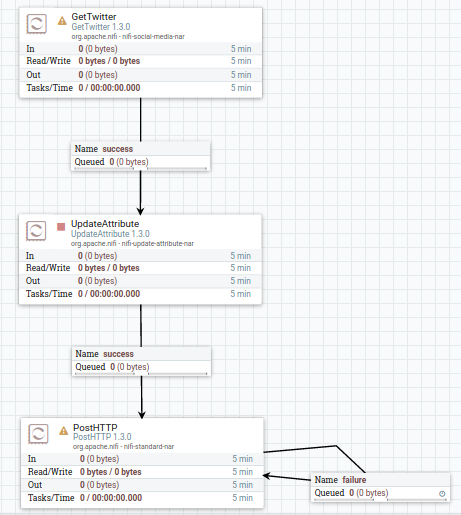
\includegraphics[width=0.7\textwidth]{nifi-tweet.png} 
    \caption{MS-Dockernifi: captura de tweets}
    \label{fig:nifi-tweet}
  \end{center}
\end{figure}

\begin{figure}[!h]
  \begin{center}
    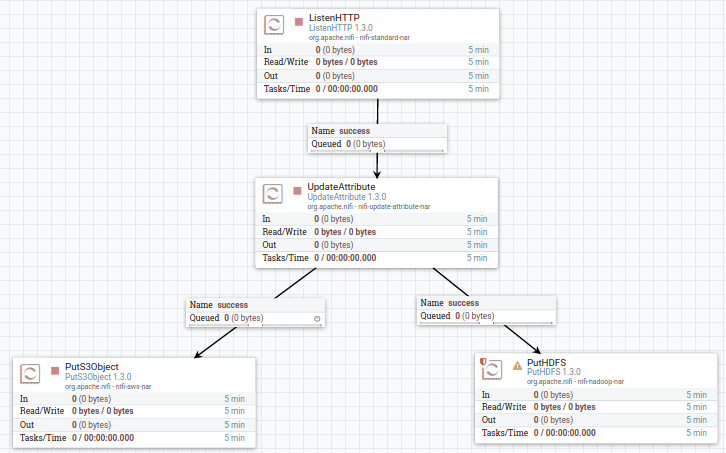
\includegraphics[width=0.7\textwidth]{nifi-ms.png} 
    \caption{MS-Dockernifi: recepción de ms.semtweet y envío a almacenamiento distribuido}
    \label{fig:nifi-ms}
  \end{center}
\end{figure}

\begin{figure}[!h]
  \begin{center}
    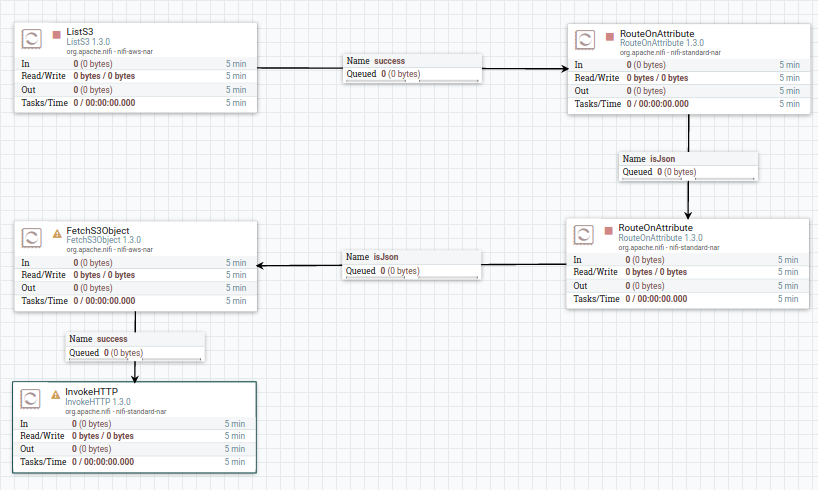
\includegraphics[width=0.7\textwidth]{nifi-s3.png} 
    \caption{MS-Dockernifi: captura de S3 y envío a ElasticSearch}
    \label{fig:nifi-s3}
  \end{center}
\end{figure}


\subsubsection{Ontología para representación de tweets: Ontotweet}

Se ha desarrollado una ontología para representar la información que contiene un
tweet en el momento que es consumido desde la \acs{API}. Esta ontología modela
las siguientes entidades: 

\begin{itemize}
\item Tweet
\item User
\item Coordinates
\item Entity $\to$ Hashstag
\end{itemize}

El resultado se puede consultar en el anexo \ref{chap:ontotwitter}.

\begin{figure}[!h]
  \begin{center}
    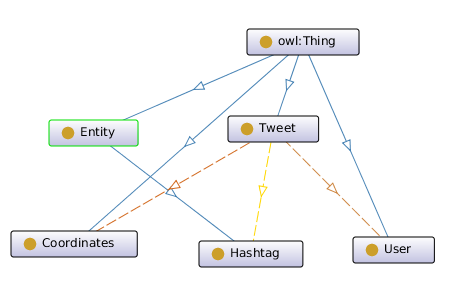
\includegraphics[width=0.6\textwidth]{ontotweet.png} 
    \caption{Esquema de la ontología de Twitter en Protégé}
    \label{fig:ontotwitterprotege}
  \end{center}
\end{figure}

\subsubsection{Microservicio de transformación de tweets: ms.semtweet}

La finalidad de este microservicio es dado un \acs{JSON} con información de un
tweet, obtener como resultado un conjunto de triplas conforme a la ontología
desarrollada en el punto anterior.

Para ello se expone una \acs{API} \acs{REST} que recibirá el tweet y enviará una
vez transformado a triplas, el resultado a un endpoint que se configurará como
parámetro en el microservicio. 

En el listado \ref{msclasses} se puede encontrar una relación entre clases en
Scala para la transformación. 

En el anexo \ref{chap:ms.semtweet} puede consultarse parte del código para
generar las triplas, mientras que en el anexo \ref{chap:ms.semtweet.docker} se muestra el DockerFile para lanzar el
microservicio. 

\lstset{escapechar=@,language=scala}
\begin{lstlisting}[caption={Entidades de transformación en Scala},captionpos=b, label=msclasses]
package org.uclm.alarcos.rrc.ms.models
case class User(id: Int, id_str: String, name: String, verified: Boolean,
                followers_count: Long, friends_count: Long,
                favourites_count: Long, created_at: String,                
                lang: String, time_zone: Option[String])
case class Coordinate(coordinates: Array[Double], `type`: String)
case class Hashtag(indices: Array[Int], text: String)
case class Entity(hashtags: Array[Hashtag])
case class Tweet (created_at: String, id: Int, id_str: String, text: String,
                  source: String, truncated: Boolean,
                  retweet_count: Long, favorite_count: Long, lang: String,
                  timestamp_ms: String, user: User, coordinates:
                  Option[Coordinate], entities: Entity)
\end{lstlisting}


\subsubsection{Servicios cloud}
\label{res:cloud}
Se han contratado para la \acs{PoC} los siguientes servicios de Amazon Web
Services: 

\begin{itemize}
\item Amazon S3: como almacenamiento escalable y distribuído. Existirán tres
  directorios principales: 
  \begin{itemize}
  \item \texttt{poc-tfm-nifi}: como directorio para el almacenamiento de tweets
    semánticos, es decir, tras haber sido procesados por ms.semtweet.
  \item \texttt{spark-sem-dq-assessment}: destino de los archivos de salida del
    job de Spark de la \acs{PoC}, organizado como sigue:
    \begin{itemize}
    \item SchemaAssessment: resultados para las evaluaciones de
      \textit{SchemaCompleteness}. 
    \item InterlinkingAssessment: resultados para las evaluaciones de \textit{Interlinking}.
    \item DQAssessmentStatistics: resultados estadísticos para cualquiera de las
      dos evaluaciones anteriores. 
    \end{itemize}
  \end{itemize}
\item ElasticSearch y Kibana: como capa de baja latencia para el consumo de
  resultados de evaluaciones y visualización. Se han creado los siguientes
  índices:

  \begin{itemize}

  \item \texttt{twittertfm}: indexará todos los tweets en bruto tal y como se
    obtienen de la \acs{API} de Twitter, sin procesar. 

  \item \texttt{interlinkingassessment}: resultados para las evaluaciones de
    \textit{Interlinking}. 
  \item \texttt{schemaasssessment}: resultados para las evaluaciones de
    \textit{SchemaCompleteness}.
  \item \texttt{dqassessmentstatistics}: resultados estadísticos para cualquiera
    de las dos evaluaciones anteriores. 
  \end{itemize}

\item Se puede consultar un ejemplo de la visualización en Kibana para la
  ingesta de tweets en bruto y resultados agregados de evaluaciones en las figuras
  \ref{fig:es-twitter} y \ref{fig:es-assessment} respectivamente. 

\end{itemize}

El diagrama final de secuencia se puede consultar en la figura \ref{fig:sequence}.

\begin{figure}[!h]
  \begin{center}
    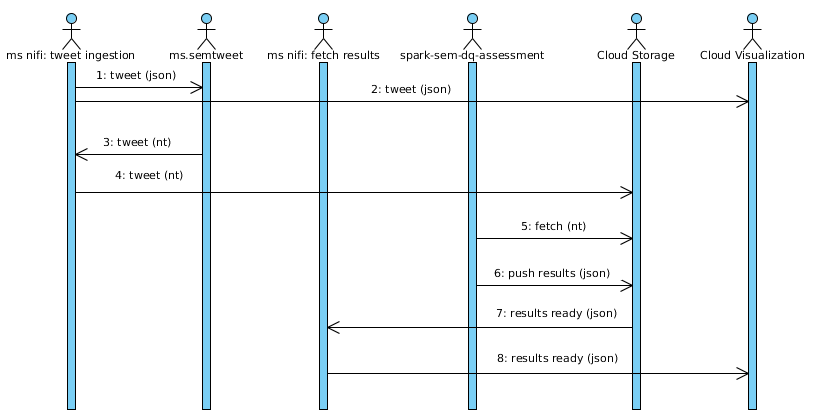
\includegraphics[width=1.2\textwidth]{sequence.png} 
    \caption{Diagrama de secuencia para la \acs{PoC}}
    \label{fig:sequence}
  \end{center}
\end{figure}


\begin{figure}[!h]
  \begin{center}
    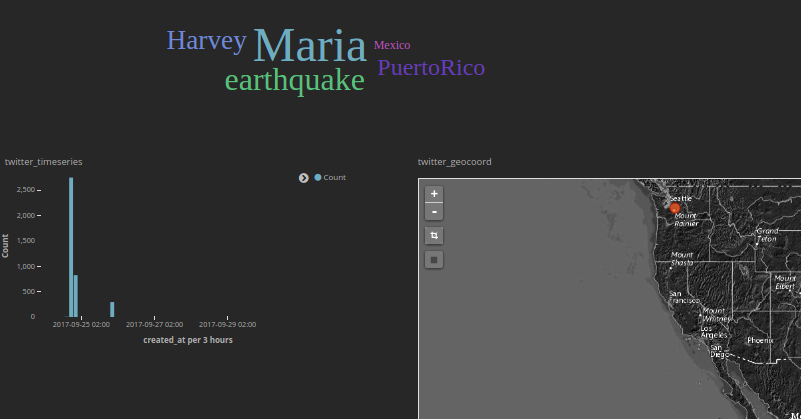
\includegraphics[width=0.6\textwidth]{tweetes.png} 
    \caption{Visualización: índice con tweets en bruto}
    \label{fig:es-twitter}
  \end{center}
\end{figure}

\begin{figure}[!h]
  \begin{center}
    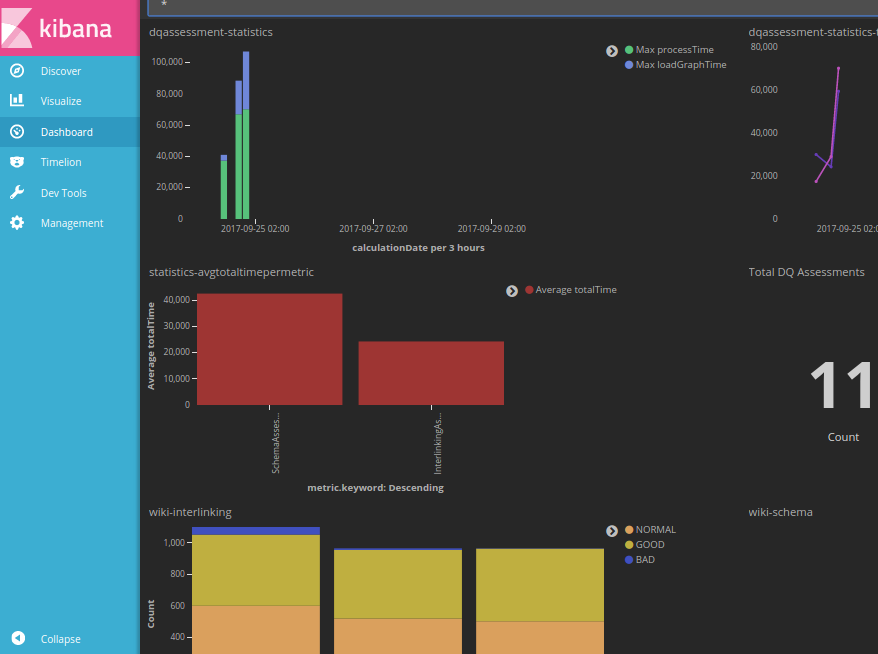
\includegraphics[width=0.6\textwidth]{assessment.png} 
    \caption{Visualización: índice con resultados de la evaluación}
    \label{fig:es-assessment}
  \end{center}
\end{figure}


\subsection{Iteración 7: Comparativa de rendimientos entre JenaDQ y SparkDQ}
\label{comparativa}

A continuación se va a exponer una comparativa entre los resultados obtenidos
ene el procesamiento de las métricas en JenaDQ y en SparkDQ. Se pueden consultar
en las tablas \ref{tab-jenadq} y \ref{tab-sparkdq}. En la tabla \ref{tab-jenadq}
se evalúa la eficiencia del cálculo de las métricas para Interlinking
considerando los dos tipos de algoritmos desarrollados para las consultas:
declarativo e iterativo (véase
\cite{PFC}). Mientras, en la tabla \ref{tab-sparkdq} se muestran los resultados
de las evaluaciones en la \acs{PoC}. 

Se puede observar cómo la diferencia de tiempos es notable ante un número de nodos mayor. 

\vspace{1cm}
Sin embargo conviene considerar los siguientes factores: 

\begin{itemize}
\item JenaDQ en sus dos algoritmos, debido al número de triplas contenido en un
  grafo semántico, consulta contra un endpoint \acs{SPARQL} a la hora de
  recuperar nuevas triplas. Esto produce un sobrecargo en el tiempo de cálculo
  cada vez que se expanden nodos. 
\item No obstante, no sería posible procesar de manera centralizada tal volumen
  de datos, pues se valora en millones de triplas, con lo cual es necesario
  consultar a un servicio remoto. 
\item SparkDQ permite una escalabilidad horizontal virtualmente ilimitada, en
  tanto que cuantos más nodos y más memoria sea asignada a los jobs de Spark que
  utilicen el stack, se podrá optimizar el tiempo y escalar de manera
  indefinida. Existen variaciones en los tiempos de carga de los datos (véase
  tabla \ref{tab-sparkdq}, para evaluaciones de Schema, el salto entre los 10k y
  70k nodos a la hora de procesar el grafo). Esto es debido al posible
  \textit{swapping} que los nodos deban hacer al ver llena la memoria. Esta
  ejecución se ha realizado aprovechando los núcleos de una sola máquina. 
\item Con estas consideraciones, cabe afirmar que la eficiencia y
  necesidad de SparkDQ queda de manifiesto ante la diferencia de al menos dos
  órdenes de magnitud a la hora del procesado de las triplas. 
\end{itemize}

% COMPLETENESS
\vspace{1cm}
\label{tab-jenadq}
\begin{tabular}{|p{.2\textwidth}|p{.12\textwidth}|p{.12\textwidth}|p{.1\textwidth}|p{.1\textwidth}|p{.2\textwidth}|}
  \tabheadformat
  \tabhead{Evaluation}         &
  \tabhead{Depth}       &
  \tabhead{Nodes} &
  \tabhead{T. Nodes}   &
  \tabhead{T. Total}  &
  \tabhead{Algorithm}   \\
\hline
:Manakkara    & 3   & 129   & 0.61s   & 11.94s  & Declarative \\
\hline
:Manakkara    & 3   & 129   & 5.51s   & 16.61s  & Iterative \\
\hline
:Life\_of\_Pi    & 3   & 11.460    & 17.45s   & 183.83s  & Declarative \\
\hline
:Life\_of\_Pi    & 2   & 1.408    & 1.903s   & 120.085s  & Declarative \\
\hline
:Metallica    & 2   & 3.897    & 5.863s   & 330.864s  & Declarative \\
\hline
:Metallica    & 1   & 229    & 0.4s   & 25.821s  & Declarative \\
\hline
:Metallica    & 1   & 229    & 0.342s & 22.672s  & Iterative \\
\hline

\end{tabular}
\captionof{table}{Resultados de procesamiento JenaDQ para tres entidades}


% Local variables:
%   coding: utf-8
%   ispell-local-dictionary: "castellano8"
%   TeX-master: "main.tex"
% End:

% COMPLETENESS
\vspace{1cm}
\label{tab-sparkdq}
\begin{tabular}{|p{.2\textwidth}|p{.1\textwidth}|p{.1\textwidth}|p{.1\textwidth}|p{.1\textwidth}|p{.2\textwidth}|}
  \tabheadformat
  \tabhead{Evaluation}   &
  \tabhead{Depth}       &
  \tabhead{Nodes} &
  \tabhead{T LoadGraph}   &
  \tabhead{T Proc}  &
  \tabhead{T Total}   \\

\hline
Interlinking    & 3   & 151 &  1.08s & 14.82s  & 15.9s \\
\hline
Interlinking    & 3   & 17.441 &  3.56s & 37.3s  & 40.88s \\
\hline
Schema      & \xmark   & 151 &  1.17s & 4.12s  & 5.29s \\
\hline
Schema      & \xmark   & 9.488 &  12.76s & 21.11s  & 33.88s \\
\hline
Schema      & \xmark   & 70.139 &  39.92s & 70.18s  & 107.11s \\
\hline
\end{tabular}
\captionof{table}{Resultados de procesamiento SparkDQ Interlinking para grafo de ejemplo}


% Local variables:
%   coding: utf-8
%   ispell-local-dictionary: "castellano8"
%   TeX-master: "main.tex"
% End:


\subsection{Iteración 8: Entrega de TFM}

% Iteración 8
\vspace{1cm}
\begin{tabular}{|p{.4\textwidth}|p{.4\textwidth}|}

\hline

\cellcolor[gray]{0.7}Fase del \acs{PUD} & Transición
 \\
\hline

\cellcolor[gray]{0.7}Flujo de trabajo del \acs{PUD} & Documentación

 \\
\hline


\cellcolor[gray]{0.7}Objetivos  &
\cellcolor[gray]{0.7}Artefactos de Salida \\
\hline

\begin{itemize}
\item Elaboración de la documentación para los distintos artefactos (SparkRDF, SparkDQ)
\item Elaboración de la documentación para la \acs{PoC}
\item Documentación \acs{TFM}
\end{itemize}

&

\begin{itemize}
\item Documentación artefactos
\item Documentación \acs{PoC}
\item Documentación \acs{TFM}
\end{itemize}
\\
\hline
\end{tabular}
\captionof{table}{Iteración 8}


% Local variables:
%   coding: utf-8
%   ispell-local-dictionary: "castellano8"
%   TeX-master: "main.tex"
% End:


La última de las iteraciones ha consistido en un trabajo de documentación
detallado de todos los pasos que han tenido lugar para la elaboración del
presente trabajo, dando como resultado los siguientes elementos: 

\begin{itemize}
\item Memoria del \acs{TFM}.
\item ScalaDoc de SparkRDF y SparkDQ.
\item Anexos.
  \begin{itemize}
  \item Ontología de tweets.
  \item Ontología \acs{DQ}.
  \item Anexo de \acs{QA}.
  \end{itemize}
\item Vídeo demostración de la \acs{PoC}.
\end{itemize}

La totalidad de la memoria ha sido realizada en \LaTeX, mientras que la
documentación de las diferentes \acs{API}s se ha generado con ScalaDoc, análogo
a JavaDoc. 

Todos los archivos de ontologías han sido incluidos en la documentación. 
